\documentclass[12pt, letterpaper]{article}
\title{CS440 Assignment1}
\author{Yuege Zhang [NetId:yz834] [Section:07]\\Samuel Kappala [NetId:sk2175] [Section:01] \\Abhishek Lyer [NetId:ami80] [Section:05]}
\date{}
\usepackage{amsmath}
\usepackage{graphicx}
\graphicspath{{./images/}}
\begin{document}
\maketitle

\section{Task A: Create the interface}
Test Image of the interface:\\
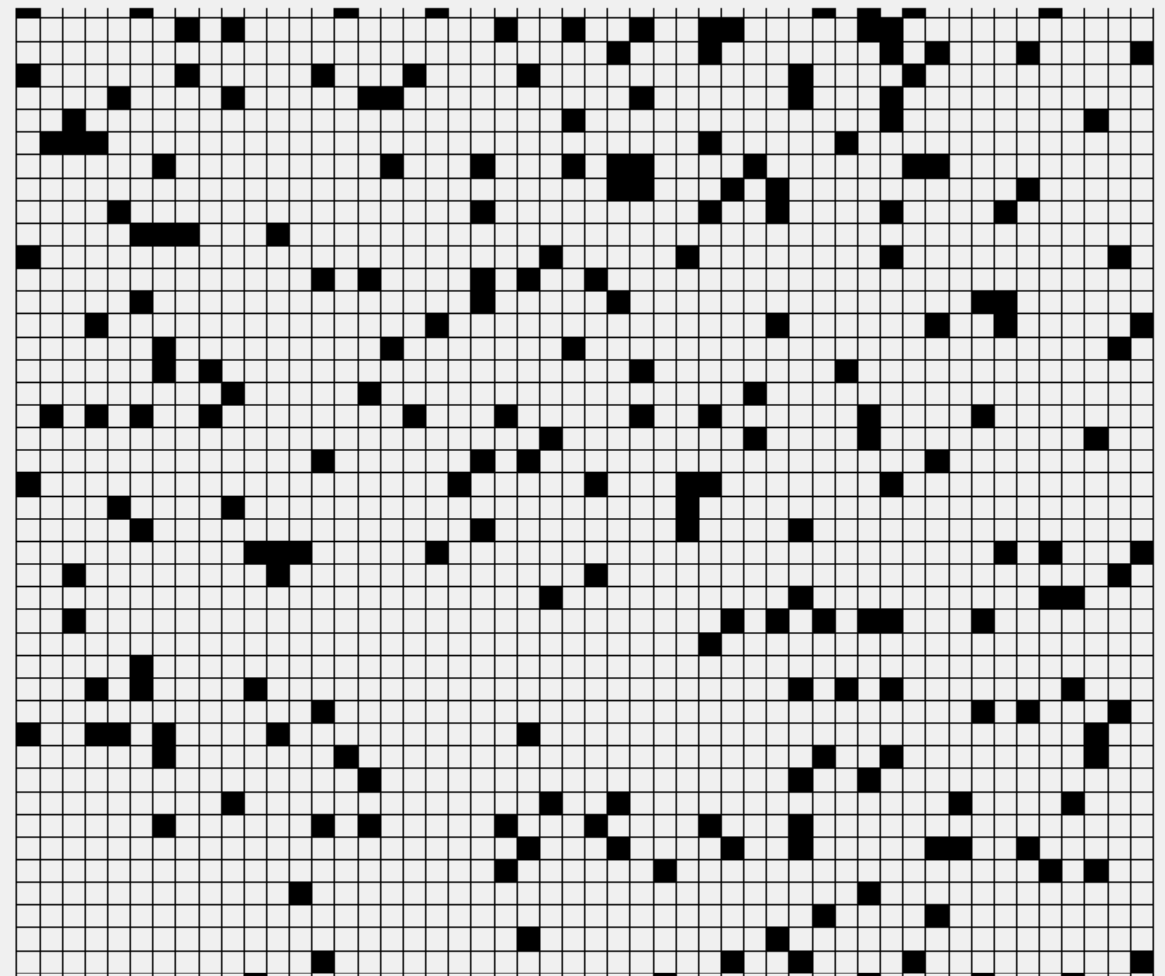
\includegraphics[width=10cm]{1a-gridtest}\\
\textbf{Capabilities:}\\
Our interactive interface is capable of generating $nxm$ grid and finding the path from the start to the goal.\\
Each grid has a random probability to be blocked. The unblocked grid is white. The blocked grid is black and the path shall cross it.\\
After generating the grid, our interface is able to find the path.\\
We provide two ways to find the path. The first one uses A* algorithm to find the shortest grid path. In this path, our vertex move from one point to its neighbor vertically, horizontally, or diagonally.\\
The second one uses Theta* algorithm to find the shortest any-angle path. In this path, our vertex can move from one point to any point, despite the distance, except the blocked grid.\\
\textbf{What we implemented for visualization:}\\
After discussion, our team chose python to program.\\
When creating the interface, we build our own class and use GUI of tkinter to visualize the graph.\\
We built a create-grid class to create a txt file containing the grid information and allow users to edit it for testing. Then we built a load-grid class to generate the graph. Aside from that, we also build a zoom function that allows users to zoom in or out of the graph.\\

\section{Task B: Find the shortest path}
\textbf{Shortest Grid Path:}\\
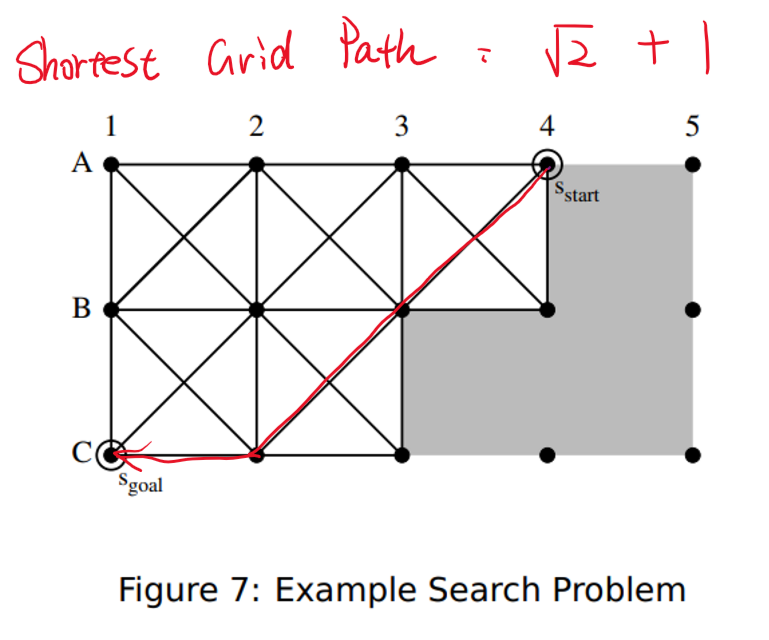
\includegraphics[width=10cm]{1b-grid}\\
\textbf{Shortest Any-angle Path:}\\
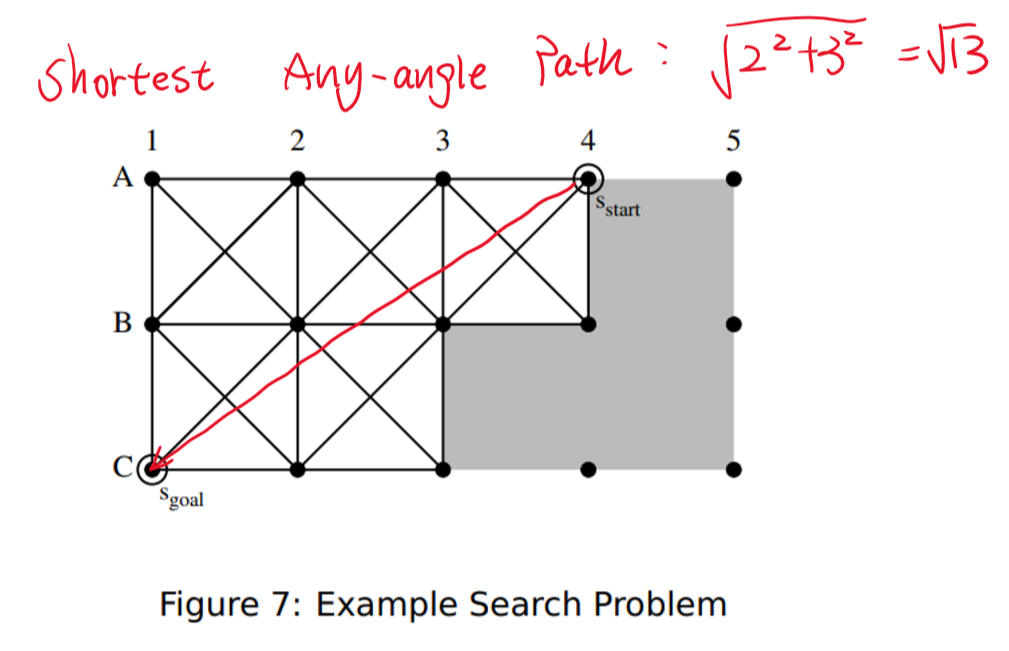
\includegraphics[width=13cm]{1b-anyangle}\\
\\
\textbf{Trace of A*:}\\
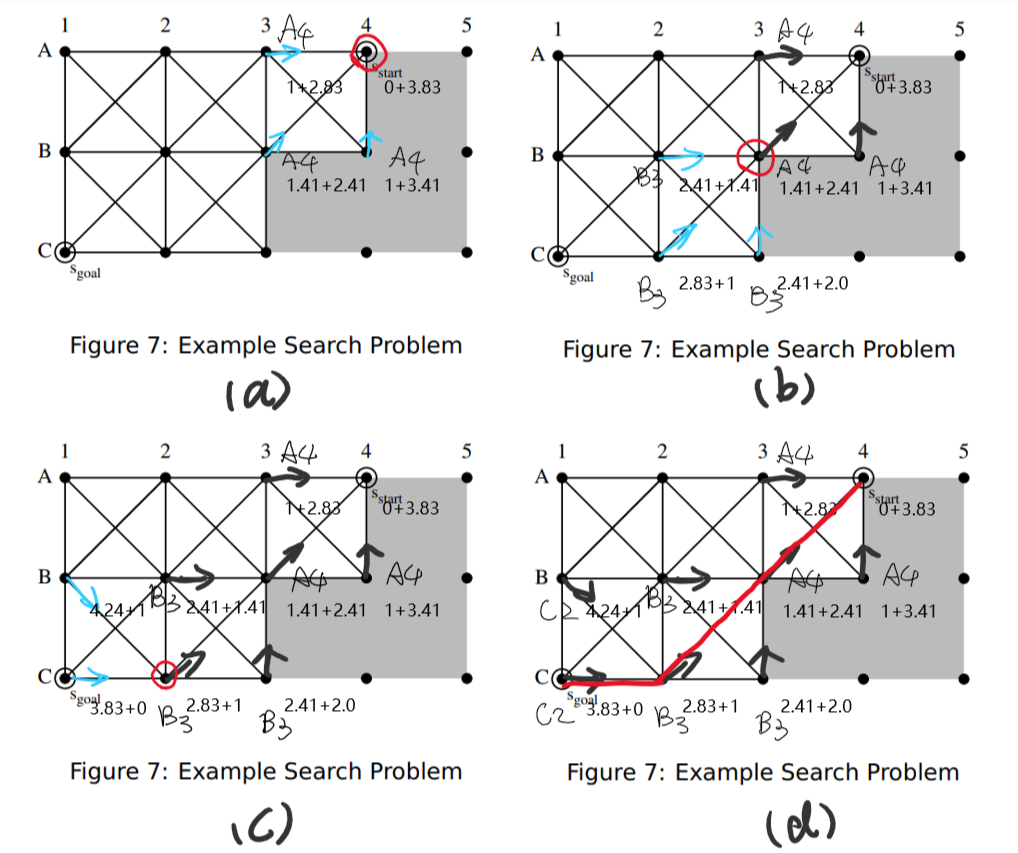
\includegraphics[width=11cm]{1b-A}\\
\textbf{Trace of Theta*:}\\
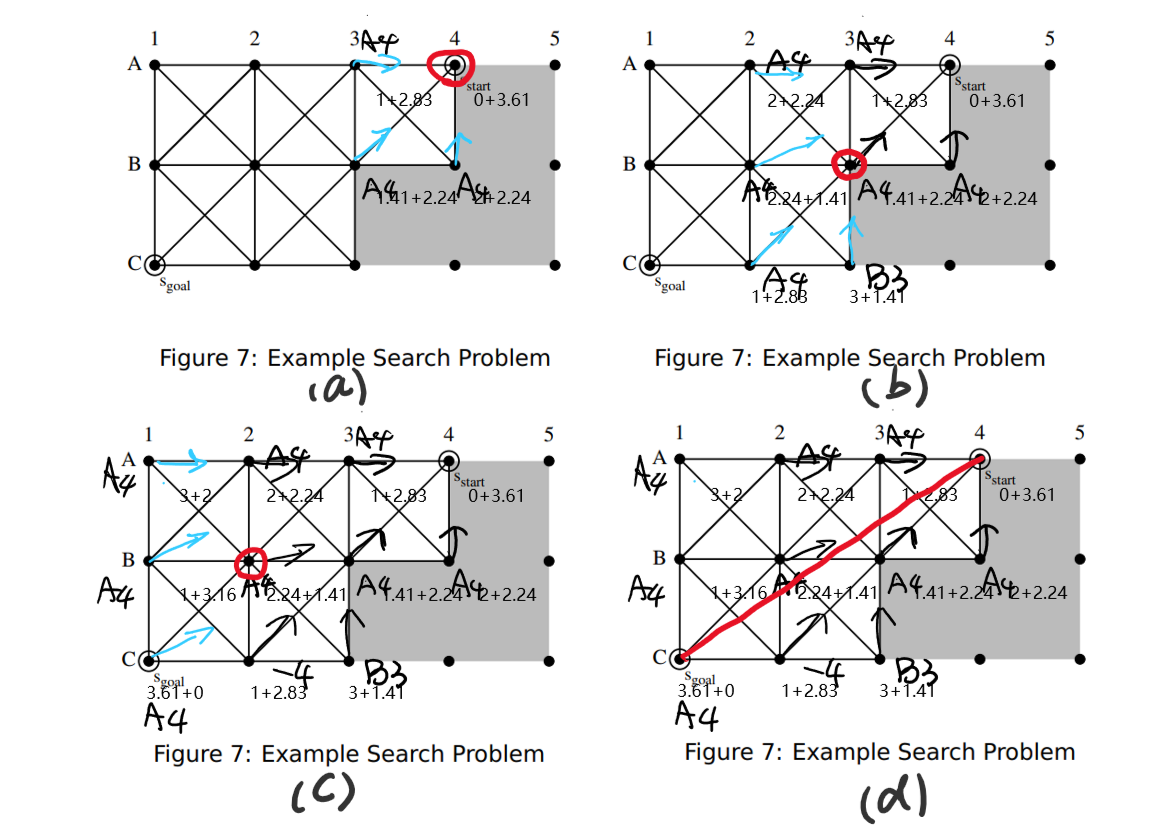
\includegraphics[width=11cm]{1b-theta}\\


\section{Task C: Implement A* algorithm}
\textbf{Test Image of A* algorithm:}\\
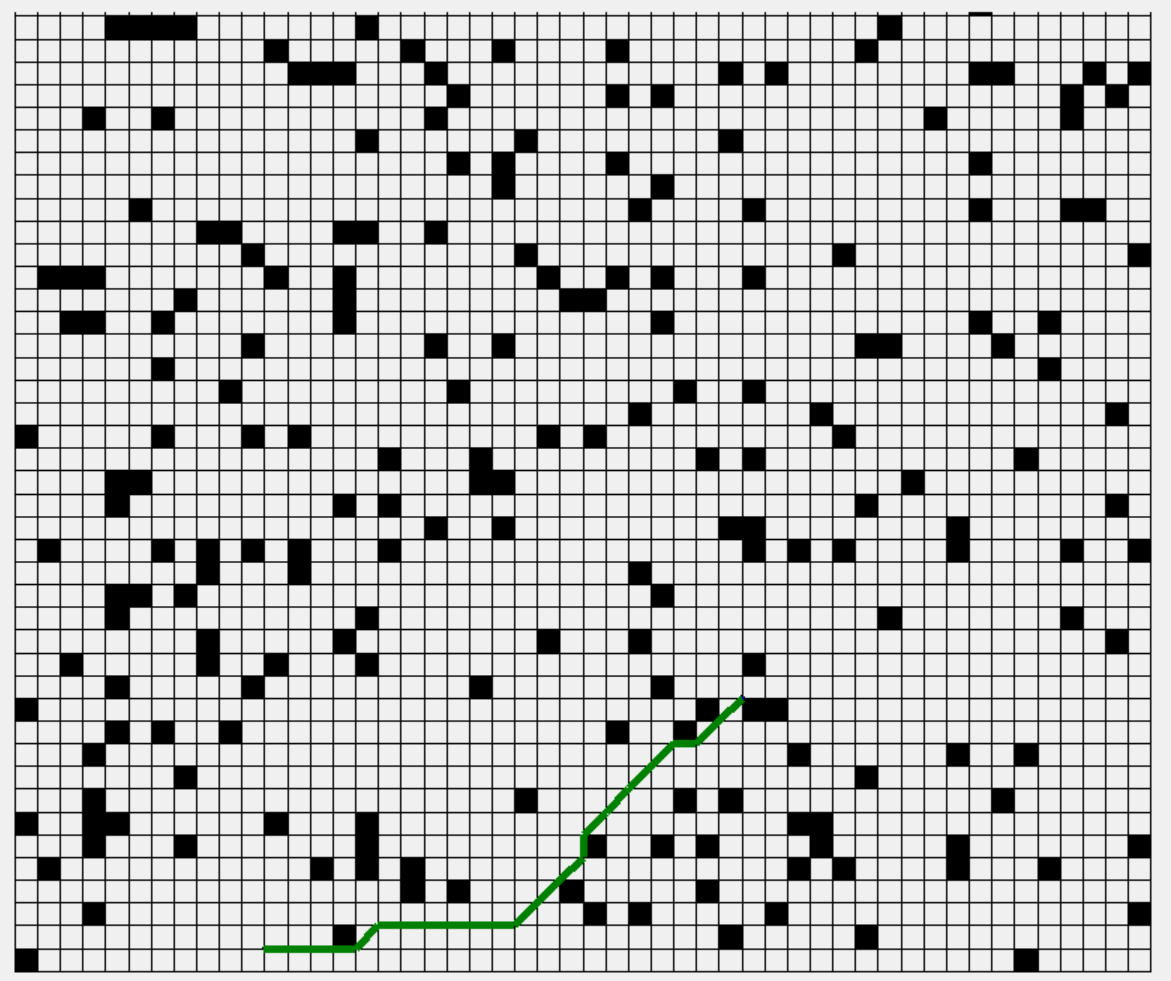
\includegraphics[width=10cm]{1c-Atest}\\
\textbf{What we had to implement to have the A* algorithm working:}\\
To get A* algorithm working, we built our own Node class. This linked list structure is the base to trace the vertexes.\\
Also, we use our own binary heap to build a function to update the node in A* algorithm.\\
Besides that, we strictly followed the A* algorithm, such as calculating g value as credentials.\\

\section{Task D: Implement Theta* algorithm}
\textbf{Test Image of Theta* algorithm:}\\
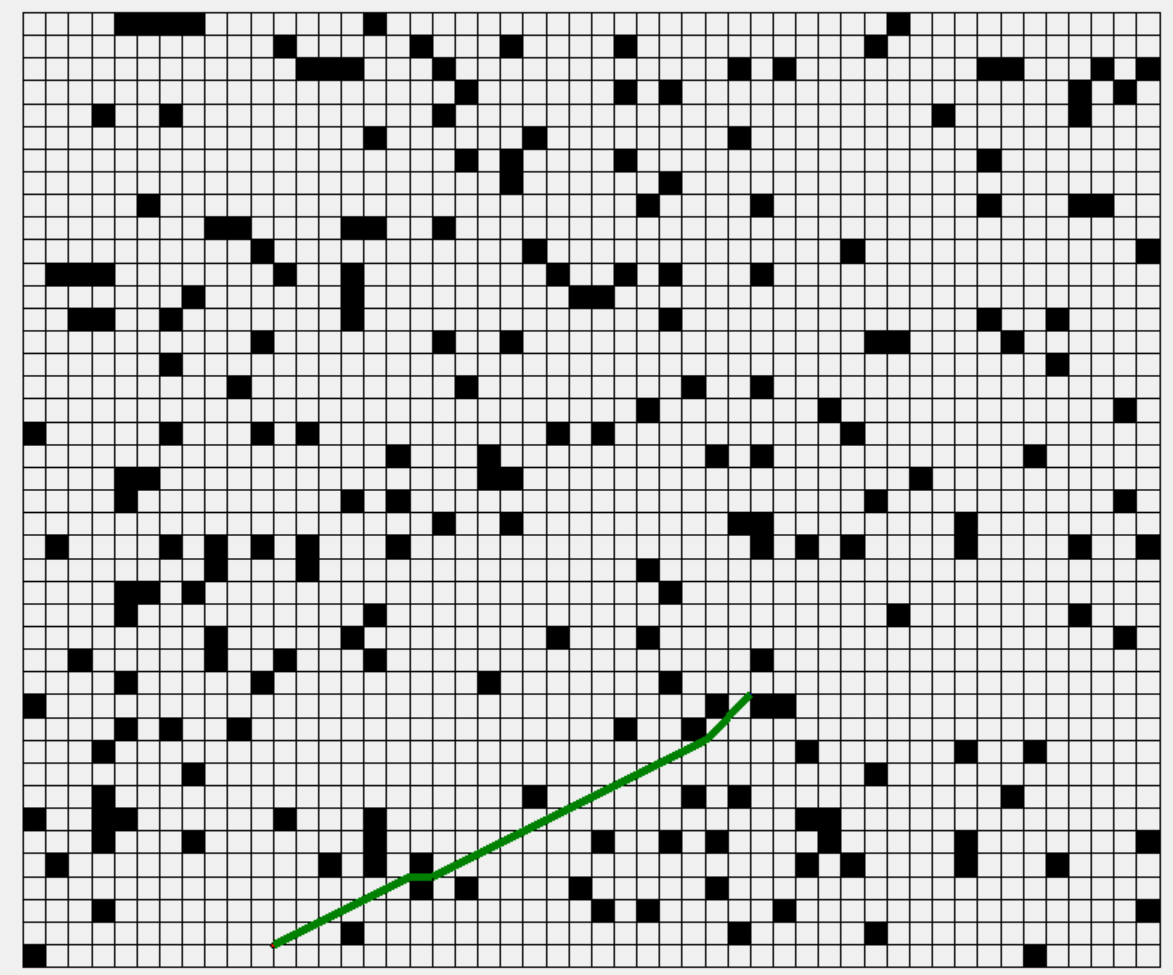
\includegraphics[width=10cm]{1c-Thetatest}\\
\textbf{What we had to implement to have the Theta* algorithm working:}\\
Similar to A* algorithm working, our own Node class is the base to trace the vertexes in Theta* algorithm.\\
The binary heap is still important in our function to update the node in Theta* algorithm.\\
Besides that, we strictly followed the Theta* algorithm, such as calculating g value as credentials.\\

\section{Task E: Proof}
We want to prove A* with the h-values from Equation 1 is
guaranteed to find shortest grid paths.\\
Equation 1:
$$h(s)=\sqrt{2} \cdot min(|s^x-s^x_{goal}|,|s^y-s^y_{goal}|) +max(|s^x-s^x_{goal}|,|s^y-s^y_{goal}|)-min(|s^x-s^x_{goal}|,|s^y-s^y_{goal}|)$$
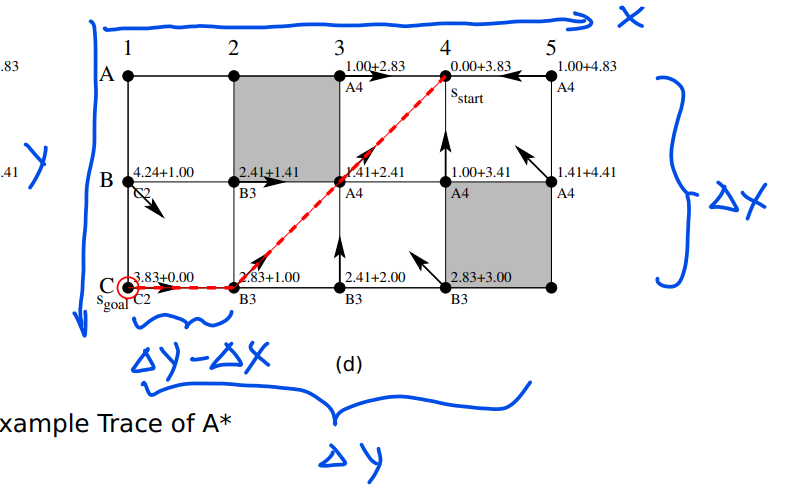
\includegraphics[width=15cm]{image-1e}\\
\textbf{Proof:}\\
We will prove it by induction.\\
Let $\Delta x=|s^x-s^x_{goal}|$ and $\Delta y=|s^y-s^y_{goal}|$\\
Then the equation is\\
$$h(s)=\sqrt 2 \cdot min(\Delta x,\Delta y)+max(\Delta x,\Delta y)-min(\Delta x,\Delta y)$$
\textbf{Base case:}\\
$\Delta x=0,\Delta y=0$\\
If the start point is the goal, $h(s)=\sqrt 2 min(0,0)+max(0,0)-min(0,0)=0$.
Since the length of path should be 0, the equation is true for the base case.\\
\textbf{Induction:}\\
Suppose this equation is true for $\Delta x=k,\ \Delta y=m$\\
To prove this equation is true for $\Delta x=k\ and\ k+1,\ \Delta y=m\ and\ m+1$:\\
We have 
$$h(s)=\sqrt 2 \cdot min(k,m)+max(k,m)-min(k,m)$$
By setting $\Delta x=k+1,\ \Delta y=m+1$, we are saying the new goal $s*$ is at diagonal of the old goal $s$.\\
The shortest path is through diagonal. And the shortest length of the path is $h(s)+\sqrt 2$. \\
\begin{align*}
h(s*)&=\sqrt 2 \cdot min(k,m)+max(k,m)-min(k,m)+\sqrt 2\\
     &=\sqrt 2 \cdot min(k+1,m+1)+max(k+1,m+1)-min(k+1,m+1)
\end{align*}
By setting $\Delta x=k,\ \Delta y=m+1$, or $\Delta x=k+1,\ \Delta y=m$, we are say the new goal $s*$ is at the direct left, right, up, or down of the old goal $s$.\\
The shortest path is through horizontal or vertical. And the shortest length of the path is $h(s)+\sqrt 2-1$. \\
\begin{align*}
h(s*)&=\sqrt 2 \cdot min(k,m)+max(k,m)-min(k,m)+\sqrt 2-1\\
     &=\sqrt 2 \cdot min(k,m+1)+max(k,m+1)-min(k,m+1)
\end{align*}
Or,
\begin{align*}
h(s*)&=\sqrt 2 \cdot min(k,m)+max(k,m)-min(k,m)+\sqrt 2-1\\
     &=\sqrt 2 \cdot min(k+1,m)+max(k+1,m)-min(k+1,m)\\
\end{align*}
Thus by induction, the equation is true for all $\Delta x$ and $\Delta y$.\\

\section{Task F: Implement our own binary heap and use it in both algorithms}
As we explained in the implementation of A* and Theta* algorithm, the binary heap is used for updating the vertexes in both algorithms.


\end{document}